\section{DUCATI: Combining DRAM-TLBs \newline and UCAT}
\label{sec:DUCATI}

\noindent UCAT and DRAM-TLB independently improve on-die processor TLB
coverage and LLT miss overhead respectively. These mechanisms can be
combined to collectively improve processor performance. To this end,
we propose {\em DUCATI}, an address translation architecture that
combines \underline{D}RAM-TLBs and \underline{UCAT-I}. While DUCATI
can either be architected with Stacked-TLBs or with SYSMEM-TLBs, we
limit our analysis of DUCATI to Stacked-TLBs. This is becuase stacked
memory technology provides better bandwidth and latency than with
conventional DDR memory technology.

\subsection{DUCATI Performance}

\begin{figure}[tp] 
\vspace{-0 in} \centering
\centerline{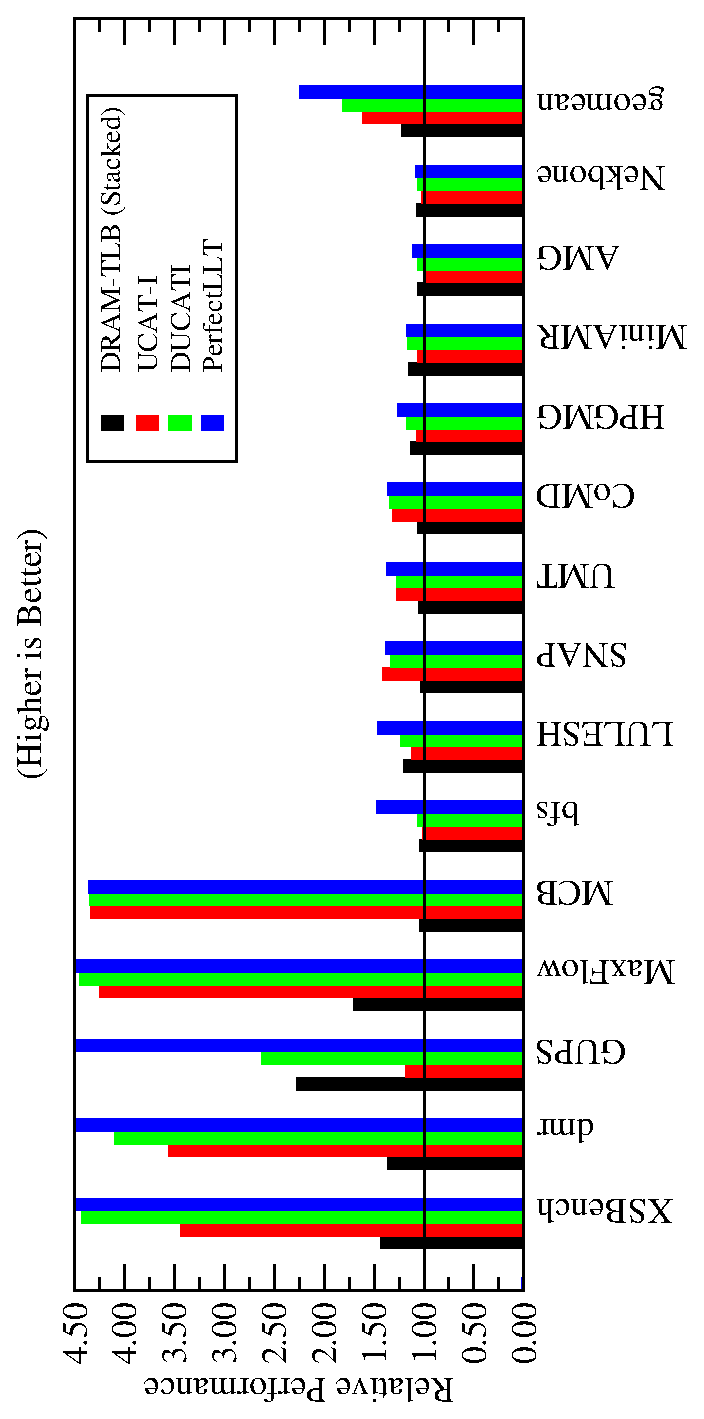
\psfig{file=GRAPHS/SUMMARY_perf,angle=-90,width=\columnwidth}}

\caption{\small Performance Summary (4KB page size).\normalsize}
\label{fig:summary_4k_pages_perf} 
\vspace{0.1 in}
\end{figure}

\begin{figure}[tp] 
\vspace{0.1 in} \centering
\centerline{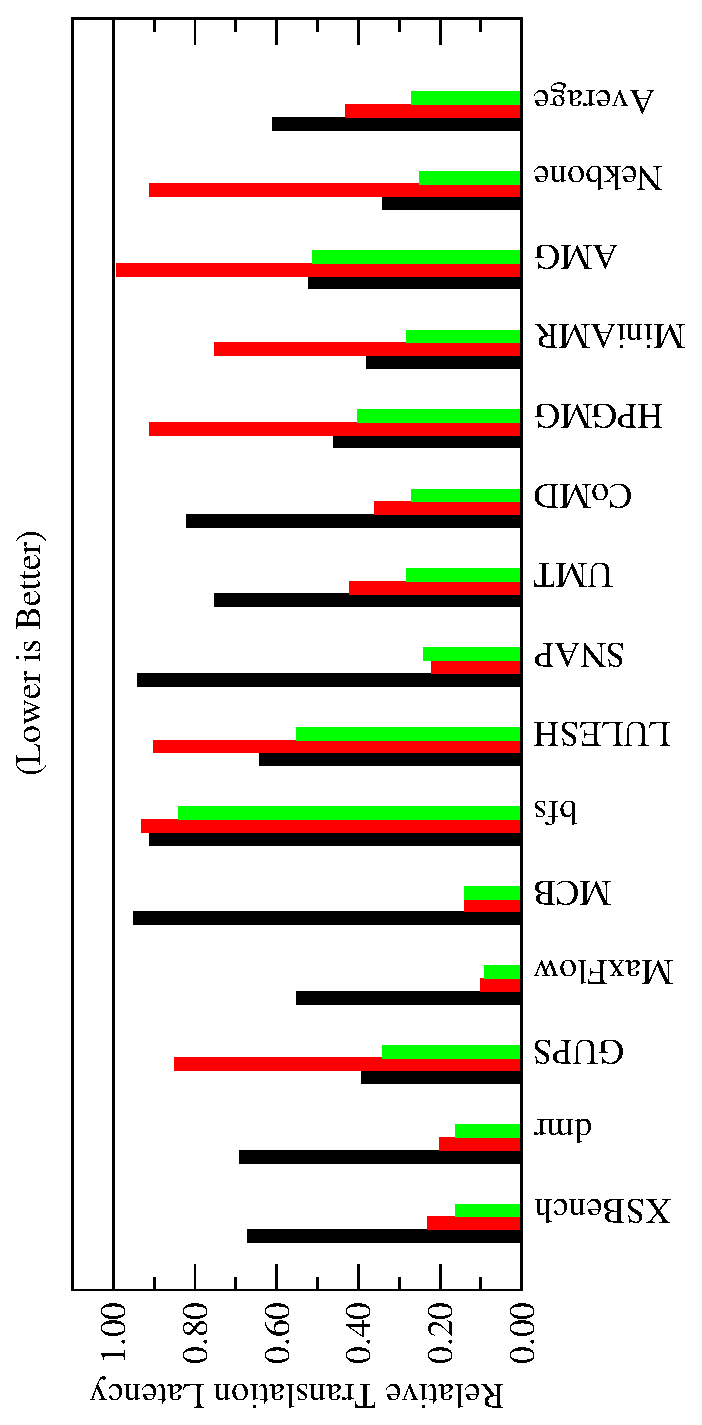
\psfig{file=GRAPHS/SUMMARY_tlblat,angle=-90,width=\columnwidth}}

\caption{\small Translation Latency (4KB page size) (same legend as
  Figure~\ref{fig:summary_4k_pages_perf}).\normalsize}
\label{fig:summary_4k_pages_lat} 
\vspace{-0. in}
\end{figure}

\noindent Figure~\ref{fig:summary_4k_pages_perf} illustrates the
relative performance of our proposals to the baseline system. The
x-axis shows the different workloads while the y-axis illustrates
performance. For each workload, we present the relative performance
for DRAM-TLBs architected with stacked memory (i.e. Stacked-TLB),
Unified Cache and TLB (UCAT) enhanced with insertion (UCAT-I), DUCATI,
and for comparison a hypotehtical Perfect LLT system\footnote{We model
a Perfect LLT by assuming all references to the LLT in the baseline
system are hits}. To provide insight into the reason for performance
improvement, Figure~\ref{fig:summary_4k_pages_lat} presents relative
address translation latencies of the different proposals.

Figure~\ref{fig:summary_4k_pages_perf} shows that stacked memory DRAM-TLBs
improve average performance by 22\%,
UCAT with insertion (UCAT-I) improves average performance by 61\%,
while DUCATI combines the benefits of both to improve average
performance by 81\%. In fact, workloads like $XSBench$, $dmr$,
$MaxFlow$, and $MCB$ experience 4x or more performance improvement.
The bulk of the gain for these workloads is improvements in on-die LLT
coverage. On the other hand, $GUPS$ has a 2.5x performance primarily
due to reduction in LLT miss penalty (i.e., the DRAM-TLB component of
DUCATI). All other workloads experience performance gains between 6\%
to 35\%.

Figure~\ref{fig:summary_4k_pages_lat} illustrates the relative address
translation latency for the different proposals that show where the
performance improvements of Figure~\ref{fig:summary_4k_pages_perf}
come from. On average, DRAM-TLB and UCAT reduce address translation
latency by 40\% and 60\% respectively, while DUCATI reduces address
translation latency by 75\%. In doing so, DUCATI improves performance
by 1.81x while a perfect LLT system improves performance by 2.24x.
Thus, DUCATI bridges two-thirds of the performance gap between the
baseline system and a perfect LLT system.

% \ee{I don't see how 1.81x and 2.24x leads to 80\% of the performance
% gap being covered, it seems more like 64\% or something like that to
% me} 

% Note that Figure~\ref{fig:summary_4k_pages_lat} clearly identifies
% workloads that are are LLT capacity bound versus those workloads that
% are LLT miss penalty bound. Specifically, workloads where the first
% bar (DRAM-TLB) is lower than the second bar (UCAT) are those that
% limited by LLT miss penalty


\subsection{DUCATI Sensitivity to Page Size}

\noindent This section presents the performance of our proposals using
64KB and 2MB page sizes. For our 1024-entry baseline LLT, using 4KB
pages provides a TLB coverage of 4MB, using 64KB pages increases the
TLB coverage to 64MB, and using 2MB pages increases TLB coverage to
2GB. Note that while large page sizes improve TLB coverage,
unrestricted use of large pages can create various performance
overheads~\cite{SuperPageProblem,TwoPageSize,numa-harmful,cameo,largepagevm}.
Nonetheless, Figure~\ref{fig:summary_pagesize} illustrates the average
performance across all workloads for 4KB, 64KB, and 2MB pages.
Overall, DUCATI improves performance by 81\% with 4KB pages, 56\% with
64K pages, and 8\% with 2MB pages. In fact, DUCATI is within 20\%,
5\%, and 2\% the performance of an unrealistic perfect LLT system when
using 4KB, 64KB, and 2MB pages respectively. Thus, with both small and
large page sizes, DUCATI is able to significantly bridge gap between
the baseline system and a perfect LLT system.

\begin{figure}[tp] 
\vspace{0. in} \centering
\centerline{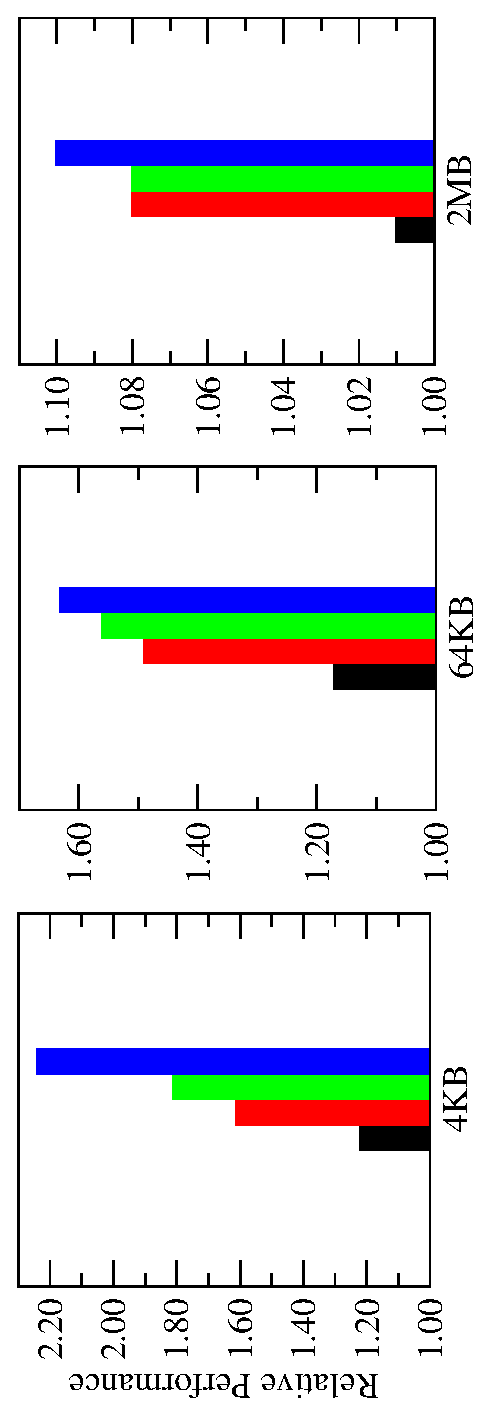
\psfig{file=GRAPHS/pagesize_sensitivity2,angle=-90,width=\columnwidth}}

\caption{\small Performance Sensitivity to Page Size (same legend as
Figure~\ref{fig:summary_4k_pages_perf}). \normalsize}

\label{fig:summary_pagesize} 
\vspace{-0. in}
\end{figure}

% \subsection{Sensitivity to Stacked DRAM Bandwidth}
% 
% \noindent Figure~\ref{fig:stack_bw_sense} illustrates the sensitivity
% of our proposals to stacked memory bandwidth. We evaluate four
% additional systems with 0.25X, 0.5X, 2X, and 4X the stacked memory
% bandwidth of the baseline system (we do not vary the system memory
% bandwidth). We increased the bandwidth by increasing the number of
% channels in the stacked memory system. The y-axis illustrates the
% average performance relative to the baseline system across all
% workloads in the study.
% 
% The figure shows that when the stacked memory bandwidth is plentiful,
% our proposals continue to improve performance. However, when the
% stacked memory bandwidth becomes a bottleneck, the memory queuing
% delays limit the performance of Distributed Placement. Under such
% scenarios, Stacked-TLBs still improve performance since they reduce
% the number of memory references. In general, our proposals efficiently
% utilize the spare bandwidth available in the stacked memory system.
% When the available bandwidth is high, performance improvements are
% high. When the available bandwidth is low, performance improvements
